%%%%%%%%%%%%%%%%%%%%%%%%%%%%%%%%%%%% Chapter Template
\chapter{Introduction} 	% Main chapter title
\label{Chapter0} 		% For referencing the chapter elsewhere, usage \ref{Chapter1}

%%%%%%%%%%%%%%%%%%%%%%%%%%%%%%%%%%%% SECTION 1
\section{Contextualisation}
\label{sec:Ch0.1}
\emph{« Ces dernières années, la conception et la production de matériel TIC "vert" et respectueux de l'environnement, ainsi que l'exploitation de services informatiques "verts", ont pris beaucoup d'importance, mais les logiciels, en tant que cause ultime des besoins en matériel et de la consommation d'énergie, n'apparaissent que lentement »}~\cite{GreenAgileMethods}. En 2013, l'article "Green Software Engineering with Agile Methods" pointait déjà du doigt cette nécessité croissante. L'avènement de la révolution numérique a transformé notre monde, plaçant les technologies de l'information et de la communication (TIC) au cœur de notre vie quotidienne. Mais cette dépendance accrue aux logiciels s'accompagne d'une ombre : une augmentation exponentielle de la consommation d'énergie, de l'empreinte carbone et de la demande en ressources, soulevant des inquiétudes environnementales majeures à l'échelle mondiale. \emph{« Les pratiques actuelles d'ingénierie logicielle ont des effets significatifs sur l'environnement. Parmi les exemples, on peut citer les déchets électroniques provenant des ordinateurs rendus obsolètes par les mises à jour logicielles, et les changements dans les besoins en énergie des nouvelles versions de logiciels.»}~\cite{TowardSustainableSoftwareEngineering} Ignorer l'impact environnemental du développement logiciel n'est plus une option. Il est impératif d'adopter des pratiques durables pour minimiser l'empreinte écologique du numérique. Ce mémoire se propose d'explorer les solutions et les meilleures pratiques pour un développement logiciel plus vert et plus responsable.

\begin{figure}[H]
    \centering
    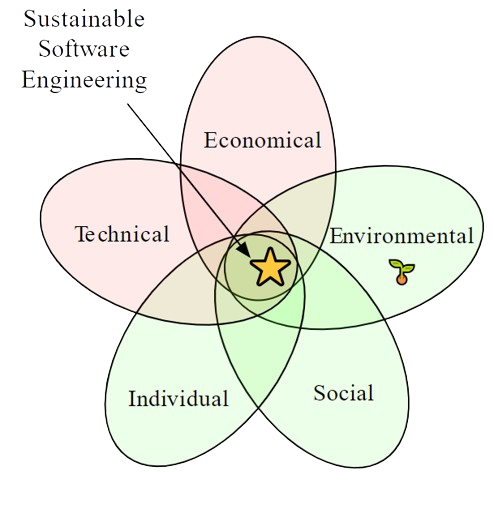
\includegraphics[width=0.4\textwidth]{MemoireMaster-NestorSkoczylas/figures/Sustainable Software Engineering.png}
    \caption{Schéma illustrant la durabilité dans le génie logiciel}
    \label{fig:durabilite-geni-logiciel}
\end{figure}

C'est dans ce contexte que s'inscrit le travail de ce mémoire, qui vise à explorer les différentes facettes de l'ingénierie logicielle durable.

%%%%%%%%%%%%%%%%%%%%%%%%%%%%%%%%%%%% SECTION 2

\section{Description du projet}
\label{sec:Ch0.2}
Ce travail de recherche s'appuie sur une approche interdisciplinaire qui combine des éléments de génie logiciel, de durabilité environnementale et de sciences sociales. 
Il vise à répondre à la questions suivante :
\begin{quote}
    
    \textit{Comment incorporer les principes de développement durable et écologique dans le processus de développement de logiciels en vue de créer des applications plus respectueuses de l'environnement ?}
    
\end{quote}

Cette proposition s'inscrit dans le cadre d'un projet plus large visant à réduire l'impact environnemental des logiciels, qui comprend plusieurs initiatives, notamment l'élaboration de lignes directrices pour l'éco-conception logicielle et la création d'un outil de mesure de l'empreinte carbone des logiciels.

%%%%%%%%%%%%%%%%%%%%%%%%%%%%%%%%%%%% SECTION 3

\section{Objectifs}
\label{sub:Ch0.3}
L'objectif principal de ce mémoire est d'explorer en profondeur les dimensions cruciales de l'ingénierie logicielle durable, mettant en lumière les défis, les opportunités, et les solutions envisageables dans ce domaine. Cette recherche aspire spécifiquement à :
\begin{itemize}
     \item Examiner de manière approfondie l'intégration efficace de la durabilité dans le processus de développement logiciel en vue de réduire son impact environnemental.
     \item Analyser l'influence des pratiques individuelles des ingénieurs logiciels sur la durabilité des produits logiciels résultants.
     \item Investiguer les pratiques durables à l'échelle globale, aussi bien au sein des projets logiciels qu'au sein des équipes de développement, tout en explorant leur cohérence avec les stratégies de la \acrfull{rse}.
\end{itemize}

Chacun de ces objectifs revêt une importance pour éclairer et contribuer à la recherche en ingénierie logicielle durable, en offrant des perspectives novatrices et des solutions concrètes.

%%%%%%%%%%%%%%%%%%%%%%%%%%%%%%%%%%%% SECTION 4
\section{Organisation du rapport}
\label{sec:Ch0.4}
Ce mémoire se compose de trois chapitres, chacun explorant un aspect distinct de la recherche sur l'ingénierie logicielle durable.

\paragraph{Chapitre \ref{mesure} : Mesure de la Durabilité dans le Développement Logiciel}
Ce chapitre examine comment évaluer et quantifier la durabilité des logiciels. Il explore d'abord la conception d'un modèle de mesure complet intégrant la durabilité dans l'évaluation des performances des projets logiciels (Section~\ref{sec:mesure-durabilite}). En suite, il analyse les approches existantes pour la pratique durable du génie logiciel, les classifiant et les évaluant dans un contexte en constante évolution (Section~\ref{sec:approches-durables}). Enfin, il examine les différentes dimensions de la durabilité conceptualisées dans la littérature académique en génie logiciel (Section~\ref{sec:dimensions-durabilite}).

\paragraph{Chapitre \ref{pratique-durabilite} : Pratiques Individuelles des Ingénieurs Logiciels et Durabilité}
Ce chapitre se concentre sur l'influence des pratiques individuelles des ingénieurs logiciels sur la durabilité des logiciels. Il explore d'abord l'impact des facteurs humains dans la conception de logiciels respectueux de l'environnement (Section~\ref{sec:pratiques-individuelles}). Ensuite, il propose des méthodes pour mesurer et améliorer la durabilité des logiciels du point de vue des pratiques individuelles des ingénieurs (Section~\ref{sec:mesure-amelioration}). Enfin, il examine comment le comportement des utilisateurs peut contribuer à la durabilité des logiciels, en soulignant l'importance de la sensibilisation et des retours d'information (Section~\ref{sec:comportement-utilisateurs}).

\paragraph{Chapitre \ref{pratique-globale} : Pratiques Durables au Niveau Global}
Ce chapitre explore les pratiques durables à l'échelle des projets et des organisations. Il examine d'abord la mise en œuvre de pratiques durables au niveau des projets logiciels, en s'appuyant sur les modèles et les outils disponibles pour évaluer et améliorer la durabilité à l'échelle du projet (Section~\ref{sec:pratiques-projets}). Ensuite, il explore comment une équipe de développement peut adopter des pratiques durables au quotidien, en identifiant les initiatives qui peuvent être mises en place pour encourager la durabilité au sein de l'équipe (Section~\ref{sec:pratiques-equipe}). Enfin, il examine comment la stratégie de \acrshort{rse} peut être alignée avec les objectifs de durabilité dans le développement logiciel, tout en abordant les avantages et les défis de l'incorporation de la durabilité dans la culture d'entreprise (Section~\ref{sec:rse-durabilite}).


Chaque chapitre est divisé en sections distinctes, chacune se concentrant sur un aspect précis du sujet. Cette structure permet une exploration approfondie de chaque thème tout en facilitant la navigation à travers le mémoire.

\section{Définition de la Durabilité}
La durabilité, la capacité à répondre \emph{« aux besoins du présent sans compromettre la capacité des générations futures à répondre aux leurs. »}~\cite{Brundtland87} 
Cette vision holistique englobe la notion de responsabilité envers l'environnement, la société, et l'économie, établissant ainsi un équilibre délicat entre les impératifs actuels et la préservation des ressources pour les générations à venir.


Dans le contexte de l'ingénierie logicielle, la durabilité va au-delà de la simple efficacité énergétique des logiciels. Elle englobe la minimisation de l'empreinte carbone, la gestion judicieuse des ressources, la prise en compte des dimensions sociales dans le processus de développement, et la création de solutions technologiques qui favorisent un équilibre harmonieux avec l'écosystème. Ainsi, définir la durabilité dans le contexte du développement logiciel revient à intégrer des principes écologiques, sociaux, et économiques au cœur même du processus de création de logiciels.


En explorant la durabilité dans le domaine du génie logiciel, ce mémoire s'engage à décortiquer ces dimensions multiples. L'analyse approfondie des pratiques individuelles des ingénieurs, la mesure de la durabilité au niveau des projets, et l'examen des implications de la \acrshort{rse} dans le développement logiciel, tous convergent vers une compréhension globale et nuancée de la durabilité dans le contexte des technologies de l'information.


Ainsi, tout au long de cette recherche, la notion de durabilité servira de fil conducteur, guidant l'exploration des défis, des opportunités, et des solutions pour forger un avenir logiciel véritablement durable. En définissant la durabilité dans ce contexte spécifique, ce mémoire aspire à contribuer à l'évolution de l'ingénierie logicielle vers des pratiques plus respectueuses de l'environnement, socialement responsables, et économiquement viables.